% Options for packages loaded elsewhere
\PassOptionsToPackage{unicode}{hyperref}
\PassOptionsToPackage{hyphens}{url}
%
\documentclass[
]{book}
\usepackage{amsmath,amssymb}
\usepackage{iftex}
\ifPDFTeX
  \usepackage[T1]{fontenc}
  \usepackage[utf8]{inputenc}
  \usepackage{textcomp} % provide euro and other symbols
\else % if luatex or xetex
  \usepackage{unicode-math} % this also loads fontspec
  \defaultfontfeatures{Scale=MatchLowercase}
  \defaultfontfeatures[\rmfamily]{Ligatures=TeX,Scale=1}
\fi
\usepackage{lmodern}
\ifPDFTeX\else
  % xetex/luatex font selection
\fi
% Use upquote if available, for straight quotes in verbatim environments
\IfFileExists{upquote.sty}{\usepackage{upquote}}{}
\IfFileExists{microtype.sty}{% use microtype if available
  \usepackage[]{microtype}
  \UseMicrotypeSet[protrusion]{basicmath} % disable protrusion for tt fonts
}{}
\makeatletter
\@ifundefined{KOMAClassName}{% if non-KOMA class
  \IfFileExists{parskip.sty}{%
    \usepackage{parskip}
  }{% else
    \setlength{\parindent}{0pt}
    \setlength{\parskip}{6pt plus 2pt minus 1pt}}
}{% if KOMA class
  \KOMAoptions{parskip=half}}
\makeatother
\usepackage{xcolor}
\usepackage{color}
\usepackage{fancyvrb}
\newcommand{\VerbBar}{|}
\newcommand{\VERB}{\Verb[commandchars=\\\{\}]}
\DefineVerbatimEnvironment{Highlighting}{Verbatim}{commandchars=\\\{\}}
% Add ',fontsize=\small' for more characters per line
\usepackage{framed}
\definecolor{shadecolor}{RGB}{248,248,248}
\newenvironment{Shaded}{\begin{snugshade}}{\end{snugshade}}
\newcommand{\AlertTok}[1]{\textcolor[rgb]{0.94,0.16,0.16}{#1}}
\newcommand{\AnnotationTok}[1]{\textcolor[rgb]{0.56,0.35,0.01}{\textbf{\textit{#1}}}}
\newcommand{\AttributeTok}[1]{\textcolor[rgb]{0.13,0.29,0.53}{#1}}
\newcommand{\BaseNTok}[1]{\textcolor[rgb]{0.00,0.00,0.81}{#1}}
\newcommand{\BuiltInTok}[1]{#1}
\newcommand{\CharTok}[1]{\textcolor[rgb]{0.31,0.60,0.02}{#1}}
\newcommand{\CommentTok}[1]{\textcolor[rgb]{0.56,0.35,0.01}{\textit{#1}}}
\newcommand{\CommentVarTok}[1]{\textcolor[rgb]{0.56,0.35,0.01}{\textbf{\textit{#1}}}}
\newcommand{\ConstantTok}[1]{\textcolor[rgb]{0.56,0.35,0.01}{#1}}
\newcommand{\ControlFlowTok}[1]{\textcolor[rgb]{0.13,0.29,0.53}{\textbf{#1}}}
\newcommand{\DataTypeTok}[1]{\textcolor[rgb]{0.13,0.29,0.53}{#1}}
\newcommand{\DecValTok}[1]{\textcolor[rgb]{0.00,0.00,0.81}{#1}}
\newcommand{\DocumentationTok}[1]{\textcolor[rgb]{0.56,0.35,0.01}{\textbf{\textit{#1}}}}
\newcommand{\ErrorTok}[1]{\textcolor[rgb]{0.64,0.00,0.00}{\textbf{#1}}}
\newcommand{\ExtensionTok}[1]{#1}
\newcommand{\FloatTok}[1]{\textcolor[rgb]{0.00,0.00,0.81}{#1}}
\newcommand{\FunctionTok}[1]{\textcolor[rgb]{0.13,0.29,0.53}{\textbf{#1}}}
\newcommand{\ImportTok}[1]{#1}
\newcommand{\InformationTok}[1]{\textcolor[rgb]{0.56,0.35,0.01}{\textbf{\textit{#1}}}}
\newcommand{\KeywordTok}[1]{\textcolor[rgb]{0.13,0.29,0.53}{\textbf{#1}}}
\newcommand{\NormalTok}[1]{#1}
\newcommand{\OperatorTok}[1]{\textcolor[rgb]{0.81,0.36,0.00}{\textbf{#1}}}
\newcommand{\OtherTok}[1]{\textcolor[rgb]{0.56,0.35,0.01}{#1}}
\newcommand{\PreprocessorTok}[1]{\textcolor[rgb]{0.56,0.35,0.01}{\textit{#1}}}
\newcommand{\RegionMarkerTok}[1]{#1}
\newcommand{\SpecialCharTok}[1]{\textcolor[rgb]{0.81,0.36,0.00}{\textbf{#1}}}
\newcommand{\SpecialStringTok}[1]{\textcolor[rgb]{0.31,0.60,0.02}{#1}}
\newcommand{\StringTok}[1]{\textcolor[rgb]{0.31,0.60,0.02}{#1}}
\newcommand{\VariableTok}[1]{\textcolor[rgb]{0.00,0.00,0.00}{#1}}
\newcommand{\VerbatimStringTok}[1]{\textcolor[rgb]{0.31,0.60,0.02}{#1}}
\newcommand{\WarningTok}[1]{\textcolor[rgb]{0.56,0.35,0.01}{\textbf{\textit{#1}}}}
\usepackage{longtable,booktabs,array}
\usepackage{calc} % for calculating minipage widths
% Correct order of tables after \paragraph or \subparagraph
\usepackage{etoolbox}
\makeatletter
\patchcmd\longtable{\par}{\if@noskipsec\mbox{}\fi\par}{}{}
\makeatother
% Allow footnotes in longtable head/foot
\IfFileExists{footnotehyper.sty}{\usepackage{footnotehyper}}{\usepackage{footnote}}
\makesavenoteenv{longtable}
\usepackage{graphicx}
\makeatletter
\def\maxwidth{\ifdim\Gin@nat@width>\linewidth\linewidth\else\Gin@nat@width\fi}
\def\maxheight{\ifdim\Gin@nat@height>\textheight\textheight\else\Gin@nat@height\fi}
\makeatother
% Scale images if necessary, so that they will not overflow the page
% margins by default, and it is still possible to overwrite the defaults
% using explicit options in \includegraphics[width, height, ...]{}
\setkeys{Gin}{width=\maxwidth,height=\maxheight,keepaspectratio}
% Set default figure placement to htbp
\makeatletter
\def\fps@figure{htbp}
\makeatother
\setlength{\emergencystretch}{3em} % prevent overfull lines
\providecommand{\tightlist}{%
  \setlength{\itemsep}{0pt}\setlength{\parskip}{0pt}}
\setcounter{secnumdepth}{5}
\usepackage{booktabs}
\ifLuaTeX
  \usepackage{selnolig}  % disable illegal ligatures
\fi
\usepackage[]{natbib}
\bibliographystyle{plainnat}
\usepackage{bookmark}
\IfFileExists{xurl.sty}{\usepackage{xurl}}{} % add URL line breaks if available
\urlstyle{same}
\hypersetup{
  pdftitle={Metod i kriminologi},
  pdfauthor={Kriminolog grupp vid Umeå universitet},
  hidelinks,
  pdfcreator={LaTeX via pandoc}}

\title{Metod i kriminologi}
\author{Kriminolog grupp vid Umeå universitet}
\date{2024-11-17}

\begin{document}
\maketitle

{
\setcounter{tocdepth}{1}
\tableofcontents
}
\chapter{Introduktion}\label{introduktion}

Vällkommen till \textbf{Kriminologi A}.

Vi bygger upp innehållet i den här boken över tid och uppdaterar den allt eftersom för att ge den bästa möjliga introduktionen till kvantitativa metoder inom kriminologi som vi kan. Vi har börjat använda R (jämfört med andra som SPSS, STATA eller Jamovi) i dessa kriminologikurser av flera anledningar. För det första tror vi att R är mer mångsidigt, vilket gör det möjligt för studenter att lära sig att använda olika statistiska verktyg som finns tillgängliga i andra program, samtidigt som de har möjlighet att tillåta andra typer av analyser som är relevanta för kriminologi (till exempel rumsliga analyser eller nätverksanalyser) som inte är tillgängliga i andra program. För det andra används R i större utsträckning inom både akademisk forskning och andra yrkesområden av intresse för studenter som studerar kriminologi, t.ex. arbete i lokala och nationella myndigheter. För det tredje är R gratis och open access, vilket innebär att det inte kommer att kosta dem pengar i framtiden att ge studenterna en introduktion till detta verktyg. För det fjärde tror vi att det finns pedagogiska fördelar som studenter får när de tvingas tänka på data och analyser med kod istället för peka-och-klicka-program. Ett exempel på detta är att kommandoraden för en linjär regressionsmodell i R är mycket lik den faktiska formeln, vilket innebär att eleverna är mer benägna att komma ihåg varje komponent i formeln tillsammans med deras betydelse. Den tänkta användningen av denna bok är att paras ihop med kriminologikurserna vid Umeå universitet och de exempel vi använder är från föreläsningarna och workshopparna i den kursen. Där det är möjligt försöker vi tillhandahålla textinformation för att förklara begreppen och hur de tillämpas i R-miljön utan att boken blir för ``texttung''.

\chapter{Set up}\label{set-up}

Här kommer instruktioner till studenter om hur att uplägga R. Följa länken och ladda när R sen ladda när Rstudio. Se till att du ladda när versionen som passar ditt dator (windows aller mac).

\url{https://posit.co/download/rstudio-desktop/}

Efter du har laddat ner båda öppen R studio gå till `file' och trycka på `ny projekt'.

\section{Packages}\label{packages}

När man först installera R eller när man uppdatera R man behöver installera paketen (packages) som vi använder att hjälpa bearbata visualisera samt analysera data. Att installera dessa packater kopiera och klistra in den följande kod och trycka `enter'. Det finns hur många som helst paketen i R som byggdes upp att göra många olika saker. I allmänhet om du vill göra någonting i R förmodligen det finns en packet för det.

``tidyverse'', ``rio'', ``ggmap'',``knitr'',``psych'',``emmeans'',
``sjPlot''

\chapter{Univariat analysis}\label{univariat-analysis}

Detta kapitel handlar om \emph{univariat analys} som vi diskuterade i
klassrummet.

Här ska vi prata om olika skal nivåer och hur de olika typer ser ut i
data formen. Sen börja med data data behandling och grunläggande
visualisering.

\section{Ladda in data till R}\label{ladda-in-data-till-r}

Först vi behöver ladda in data kopiera och och klistra in data. Kan du
ser datafilen i R studio? Om inte se till att du had lagt filen i samma
plats som ditt R projekt. När du har gjort den och kan se filen i R
studio då du kan trycka den gröna plus tecken högst upp i vänsterhörnet.
Kopiera och klistra in den följande kod till dina skript och kör koden.

\begin{Shaded}
\begin{Highlighting}[]
\FunctionTok{library}\NormalTok{(rio)}
\NormalTok{df}\OtherTok{\textless{}{-}}\FunctionTok{import}\NormalTok{(}\StringTok{\textquotesingle{}NTU 2017{-}2021.RData\textquotesingle{}}\NormalTok{)}
\end{Highlighting}
\end{Shaded}

\begin{verbatim}
## Warning: Missing `trust` will be set to FALSE by default for RData in 2.0.0.
\end{verbatim}

Nu du borde se en ny objekt i enrironment fönstret som heter `df' som
inkludera 375790 observationer och 6 variabler. Om du vill titta på
datan du kan trycka på den och en ny fönster ska öppna med datavy.

\section{Data överblick.}\label{data-uxf6verblick.}

Här kommer två sätt att får samma information

\begin{Shaded}
\begin{Highlighting}[]
\FunctionTok{head}\NormalTok{(df)}
\end{Highlighting}
\end{Shaded}

\begin{verbatim}
##   alder_4 Brottsoffer_hot Fortroende_index  Radsla_oro
## 1   65-84             Nej                8      Orolig
## 2   65-84             Nej               20      Orolig
## 3   65-84            <NA>                7 Inte orolig
## 4   65-84             Nej               NA Inte orolig
## 5   65-84             Nej               19      Orolig
## 6   65-84             Nej               15      Orolig
##                         Radsla_beteende      Storstad
## 1 Sällan eller aldrig avstått aktivitet Inte storstad
## 2 Sällan eller aldrig avstått aktivitet      Storstad
## 3 Sällan eller aldrig avstått aktivitet Inte storstad
## 4 Sällan eller aldrig avstått aktivitet Inte storstad
## 5                Ofta avstått aktivitet Inte storstad
## 6                Ofta avstått aktivitet Inte storstad
\end{verbatim}

\begin{Shaded}
\begin{Highlighting}[]
\NormalTok{knitr}\SpecialCharTok{::}\FunctionTok{kable}\NormalTok{(}
  \FunctionTok{head}\NormalTok{(df, }\DecValTok{10}\NormalTok{), }\AttributeTok{caption =} \StringTok{\textquotesingle{}Here is a nice table!\textquotesingle{}}\NormalTok{,}
  \AttributeTok{booktabs =} \ConstantTok{TRUE}
\NormalTok{)}
\end{Highlighting}
\end{Shaded}

\begin{table}

\caption{\label{tab:unnamed-chunk-4}Here is a nice table!}
\centering
\begin{tabular}[t]{llrlll}
\toprule
alder\_4 & Brottsoffer\_hot & Fortroende\_index & Radsla\_oro & Radsla\_beteende & Storstad\\
\midrule
65-84 & Nej & 8 & Orolig & Sällan eller aldrig avstått aktivitet & Inte storstad\\
65-84 & Nej & 20 & Orolig & Sällan eller aldrig avstått aktivitet & Storstad\\
65-84 & NA & 7 & Inte orolig & Sällan eller aldrig avstått aktivitet & Inte storstad\\
65-84 & Nej & NA & Inte orolig & Sällan eller aldrig avstått aktivitet & Inte storstad\\
65-84 & Nej & 19 & Orolig & Ofta avstått aktivitet & Inte storstad\\
\addlinespace
65-84 & Nej & 15 & Orolig & Ofta avstått aktivitet & Inte storstad\\
65-84 & Nej & NA & Orolig & Sällan eller aldrig avstått aktivitet & Storstad\\
65-84 & Nej & 6 & Inte orolig & Sällan eller aldrig avstått aktivitet & Inte storstad\\
65-84 & Nej & 14 & Orolig & Sällan eller aldrig avstått aktivitet & Inte storstad\\
65-84 & Nej & 19 & Orolig & Sällan eller aldrig avstått aktivitet & Storstad\\
\bottomrule
\end{tabular}
\end{table}

\section{Descriptive statistics}\label{descriptive-statistics}

Vi måste alltid kommer ihåg skal nivå av variablerna när vi kör alla
slags analysen. Även i univariatanalys t.ex. vad btyder det att räkna ut
medelvärdet av en dikatom variabel som `storstad'?

\begin{Shaded}
\begin{Highlighting}[]
\FunctionTok{library}\NormalTok{(psych)}
\NormalTok{knitr}\SpecialCharTok{::}\FunctionTok{kable}\NormalTok{(}\FunctionTok{describe}\NormalTok{(df))}
\end{Highlighting}
\end{Shaded}

\begin{tabular}{l|r|r|r|r|r|r|r|r|r|r|r|r|r}
\hline
  & vars & n & mean & sd & median & trimmed & mad & min & max & range & skew & kurtosis & se\\
\hline
alder\_4* & 1 & 375590 & 2.841875 & 1.0327887 & 3 & 2.927344 & 1.4826 & 1 & 4 & 3 & -0.4060423 & -1.0256244 & 0.0016852\\
\hline
Brottsoffer\_hot* & 2 & 371042 & 1.925895 & 0.2619417 & 2 & 2.000000 & 0.0000 & 1 & 2 & 1 & -3.2518225 & 8.5743727 & 0.0004300\\
\hline
Fortroende\_index & 3 & 269696 & 11.408805 & 4.5050388 & 12 & 11.625914 & 4.4478 & 0 & 20 & 20 & -0.4529712 & -0.2107235 & 0.0086748\\
\hline
Radsla\_oro* & 4 & 366123 & 1.451627 & 0.4976552 & 1 & 1.439534 & 0.0000 & 1 & 2 & 1 & 0.1944035 & -1.9622126 & 0.0008225\\
\hline
Radsla\_beteende* & 5 & 373014 & 1.117682 & 0.3222315 & 1 & 1.022104 & 0.0000 & 1 & 2 & 1 & 2.3729340 & 3.6308253 & 0.0005276\\
\hline
Storstad* & 6 & 375590 & 1.289012 & 0.4533041 & 1 & 1.236265 & 0.0000 & 1 & 2 & 1 & 0.9308872 & -1.1334520 & 0.0007397\\
\hline
\end{tabular}

\section{Visualisering}\label{visualisering}

\begin{Shaded}
\begin{Highlighting}[]
\CommentTok{\#Här är en plot av variabeln \textquotesingle{}Brottsoffer\_hot\textquotesingle{}.  }
\FunctionTok{library}\NormalTok{(tidyverse)}
\end{Highlighting}
\end{Shaded}

\begin{verbatim}
## -- Attaching core tidyverse packages ------------------------ tidyverse 2.0.0 --
## v dplyr     1.1.4     v readr     2.1.5
## v forcats   1.0.0     v stringr   1.5.1
## v ggplot2   3.5.1     v tibble    3.2.1
## v lubridate 1.9.3     v tidyr     1.3.1
## v purrr     1.0.2     
## -- Conflicts ------------------------------------------ tidyverse_conflicts() --
## x ggplot2::%+%()   masks psych::%+%()
## x ggplot2::alpha() masks psych::alpha()
## x dplyr::filter()  masks stats::filter()
## x dplyr::lag()     masks stats::lag()
## i Use the conflicted package (<http://conflicted.r-lib.org/>) to force all conflicts to become errors
\end{verbatim}

\begin{Shaded}
\begin{Highlighting}[]
\NormalTok{df }\SpecialCharTok{\%\textgreater{}\%} \FunctionTok{drop\_na}\NormalTok{() }\SpecialCharTok{\%\textgreater{}\%} \CommentTok{\#Det har ta bort alla NA annars det får sin egen kolumn}
  \FunctionTok{ggplot}\NormalTok{()}\SpecialCharTok{+} \FunctionTok{geom\_bar}\NormalTok{(}\FunctionTok{aes}\NormalTok{(}\AttributeTok{x=}\NormalTok{Brottsoffer\_hot))}\SpecialCharTok{+}\FunctionTok{theme\_bw}\NormalTok{()}
\end{Highlighting}
\end{Shaded}

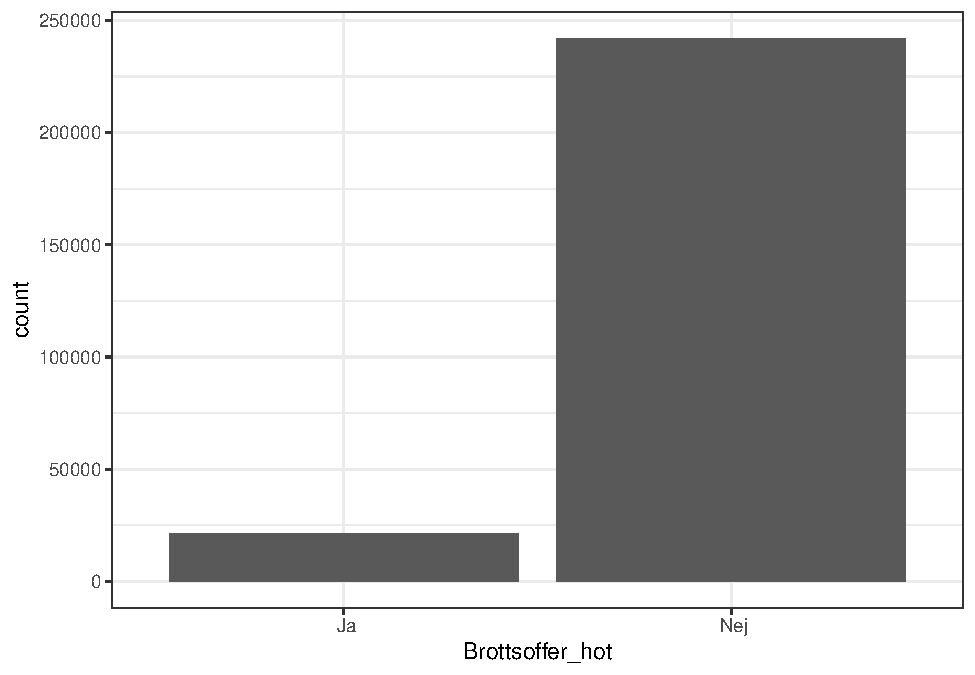
\includegraphics{_main_files/figure-latex/unnamed-chunk-6-1.pdf}

\begin{Shaded}
\begin{Highlighting}[]
\CommentTok{\#Här är en plot av variabeln \textquotesingle{}Radsla\_oro\textquotesingle{}.  }

\NormalTok{df }\SpecialCharTok{\%\textgreater{}\%} \FunctionTok{drop\_na}\NormalTok{() }\SpecialCharTok{\%\textgreater{}\%} \CommentTok{\#Det har ta bort alla NA annars det får sin egen kolumn}
  \FunctionTok{ggplot}\NormalTok{()}\SpecialCharTok{+} \FunctionTok{geom\_bar}\NormalTok{(}\FunctionTok{aes}\NormalTok{(}\AttributeTok{x=}\NormalTok{Radsla\_oro))}\SpecialCharTok{+}\FunctionTok{theme\_bw}\NormalTok{()}
\end{Highlighting}
\end{Shaded}

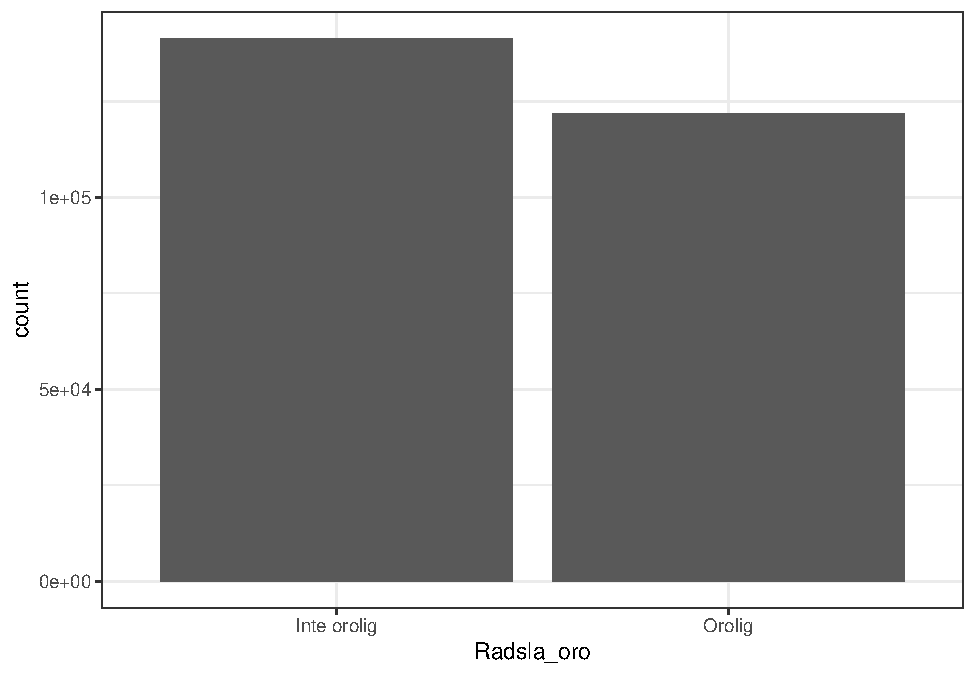
\includegraphics{_main_files/figure-latex/unnamed-chunk-7-1.pdf}

\begin{Shaded}
\begin{Highlighting}[]
\CommentTok{\#Här är en plot av variabeln \textquotesingle{}Radsla\_beteende\textquotesingle{}.  }

\NormalTok{df }\SpecialCharTok{\%\textgreater{}\%} \FunctionTok{drop\_na}\NormalTok{() }\SpecialCharTok{\%\textgreater{}\%} \CommentTok{\#Det har ta bort alla NA annars det får sin egen kolumn}
  \FunctionTok{ggplot}\NormalTok{()}\SpecialCharTok{+} \FunctionTok{geom\_bar}\NormalTok{(}\FunctionTok{aes}\NormalTok{(}\AttributeTok{x=}\NormalTok{Radsla\_beteende))}\SpecialCharTok{+}\FunctionTok{theme\_bw}\NormalTok{()}
\end{Highlighting}
\end{Shaded}

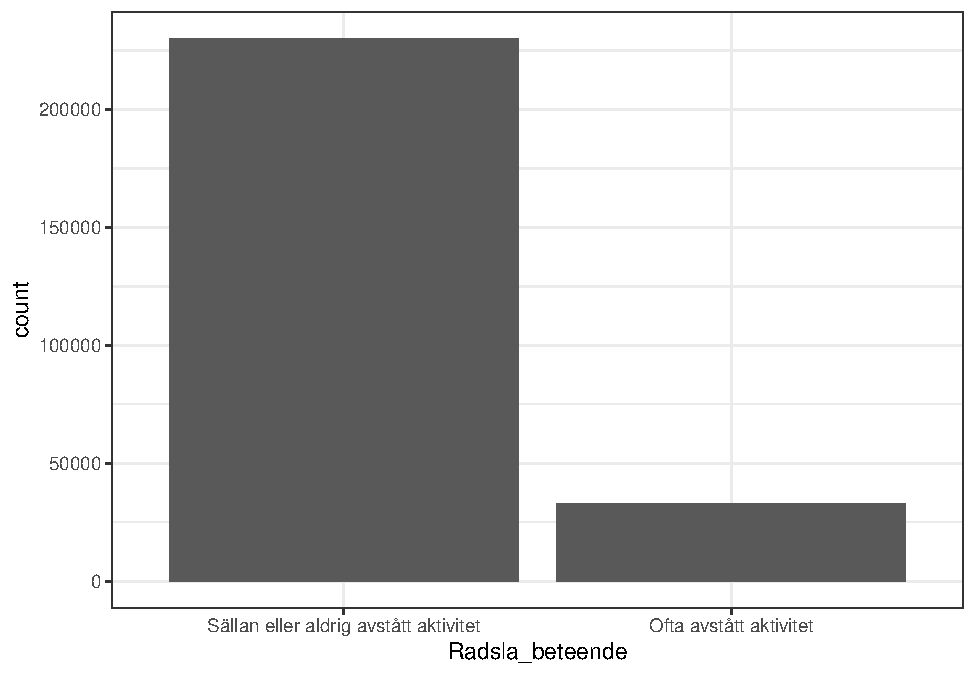
\includegraphics{_main_files/figure-latex/unnamed-chunk-8-1.pdf}

De tre variablerna var alla dikotomiserad i.e.~de variera bara mellan
två kategorier. Men vi kan också skapa en `index' av många variabler

I denna fall vi har skapat ett additivt index (en sammanslagning av fem
frågor) som mäter om respondenten har stort eller litet förtroende för
rättsväsendet. Kontinuerlig: 0 (lågt förtroende) till 20 (högt
förtroende) (Ingenåsikt/vetinte=bortfall)

Vi kan se de beskrivande statistiker för bara denna variabel om vi lägga
till variabelns namn efter datasetets namn och en `\$' tecken

\begin{Shaded}
\begin{Highlighting}[]
\NormalTok{knitr}\SpecialCharTok{::}\FunctionTok{kable}\NormalTok{(}\FunctionTok{describe}\NormalTok{(df}\SpecialCharTok{$}\NormalTok{Fortroende\_index, }\AttributeTok{skew =} \ConstantTok{FALSE}\NormalTok{))}
\end{Highlighting}
\end{Shaded}

\begin{tabular}{l|r|r|r|r|r|r|r|r|r}
\hline
  & vars & n & mean & sd & median & min & max & range & se\\
\hline
X1 & 1 & 269696 & 11.4088 & 4.505039 & 12 & 0 & 20 & 20 & 0.0086748\\
\hline
\end{tabular}

\begin{Shaded}
\begin{Highlighting}[]
\CommentTok{\#Här är en plot av variabeln \textquotesingle{}Fortroende\_index\textquotesingle{}.  }

\NormalTok{df }\SpecialCharTok{\%\textgreater{}\%} \FunctionTok{drop\_na}\NormalTok{() }\SpecialCharTok{\%\textgreater{}\%} \CommentTok{\#Det har ta bort alla NA annars det får sin egen kolumn}
  \FunctionTok{ggplot}\NormalTok{()}\SpecialCharTok{+} \FunctionTok{geom\_bar}\NormalTok{(}\FunctionTok{aes}\NormalTok{(}\AttributeTok{x=}\NormalTok{Fortroende\_index))}\SpecialCharTok{+}\FunctionTok{theme\_bw}\NormalTok{()}
\end{Highlighting}
\end{Shaded}

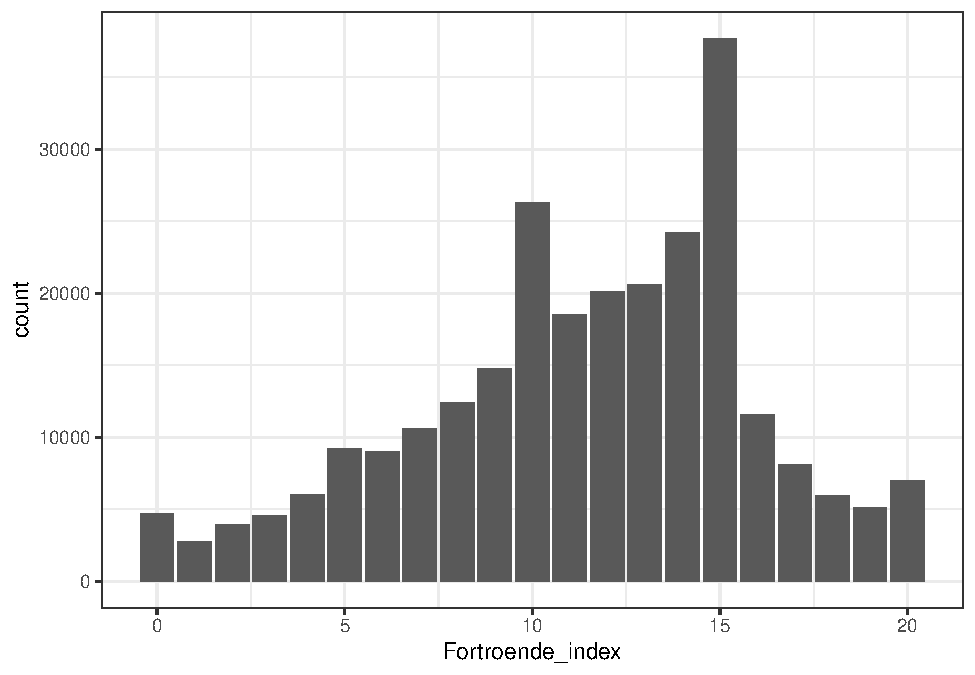
\includegraphics{_main_files/figure-latex/unnamed-chunk-10-1.pdf}

Sen vi kan även ladda upp en till data set om vi vill. Lada ner den
`shootings' excel fil från canvas och spara den i samma map som du har R
projektet. När du har gjort den det borde dycker upp i fönstret igen.
Sen kör denna kod att ladda in data till R och nämna den `shootings'

\begin{Shaded}
\begin{Highlighting}[]
\NormalTok{shootings}\OtherTok{\textless{}{-}} \FunctionTok{import}\NormalTok{(}\StringTok{\textquotesingle{}shootings.csv\textquotesingle{}}\NormalTok{)}
\CommentTok{\#Sen kolla hur det ser ut}
\FunctionTok{head}\NormalTok{(shootings)}
\end{Highlighting}
\end{Shaded}

\begin{verbatim}
##   year         region shootings_rate trust_police_average education_average
## 1 2018 västragötaland       2.982781             2.277397          2.252655
## 2 2018       blekinge       1.252474             2.430769          2.112299
## 3 2018      jönköping       2.494284             2.264463          2.113990
## 4 2018 västernorrland       0.407410             2.447059          2.180451
## 5 2018    västmanland       1.825290             2.169014          2.216000
## 6 2018   södermanland       4.411341             2.272727          2.148036
##   income_average
## 1       3.501167
## 2       3.200000
## 3       3.400552
## 4       3.315175
## 5       3.502146
## 6       3.370253
\end{verbatim}

\begin{Shaded}
\begin{Highlighting}[]
\NormalTok{knitr}\SpecialCharTok{::}\FunctionTok{kable}\NormalTok{(}\FunctionTok{describe}\NormalTok{(shootings}\SpecialCharTok{$}\NormalTok{shootings\_rate, }\AttributeTok{skew =} \ConstantTok{FALSE}\NormalTok{))}
\end{Highlighting}
\end{Shaded}

\begin{tabular}{l|r|r|r|r|r|r|r|r|r}
\hline
  & vars & n & mean & sd & median & min & max & range & se\\
\hline
X1 & 1 & 63 & 2.557833 & 1.898535 & 2.125386 & 0 & 8.860789 & 8.860789 & 0.2391929\\
\hline
\end{tabular}

\begin{Shaded}
\begin{Highlighting}[]
\NormalTok{shootings }\SpecialCharTok{\%\textgreater{}\%} \FunctionTok{drop\_na}\NormalTok{() }\SpecialCharTok{\%\textgreater{}\%} 
  \FunctionTok{ggplot}\NormalTok{(}\FunctionTok{aes}\NormalTok{(shootings\_rate))}\SpecialCharTok{+} \FunctionTok{geom\_histogram}\NormalTok{(}\AttributeTok{binwidth=}\NormalTok{ .}\DecValTok{75}\NormalTok{)}\SpecialCharTok{+}
   \FunctionTok{theme\_bw}\NormalTok{()}
\end{Highlighting}
\end{Shaded}

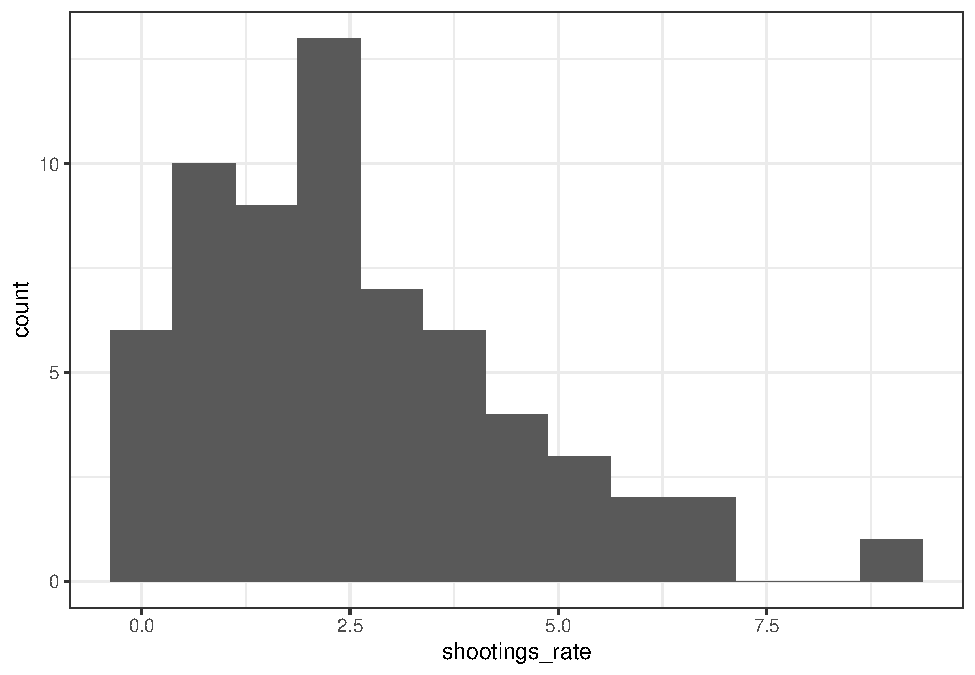
\includegraphics{_main_files/figure-latex/unnamed-chunk-13-1.pdf}

Vi kan också skapa en boxplot av variabeln

\begin{Shaded}
\begin{Highlighting}[]
\NormalTok{shootings }\SpecialCharTok{\%\textgreater{}\%} \FunctionTok{drop\_na}\NormalTok{() }\SpecialCharTok{\%\textgreater{}\%} 
  \FunctionTok{ggplot}\NormalTok{(}\FunctionTok{aes}\NormalTok{(}\AttributeTok{x=}\NormalTok{ shootings\_rate))}\SpecialCharTok{+} \FunctionTok{geom\_boxplot}\NormalTok{()}\SpecialCharTok{+} \FunctionTok{coord\_flip}\NormalTok{()}\SpecialCharTok{+} \FunctionTok{theme\_bw}\NormalTok{()}
\end{Highlighting}
\end{Shaded}

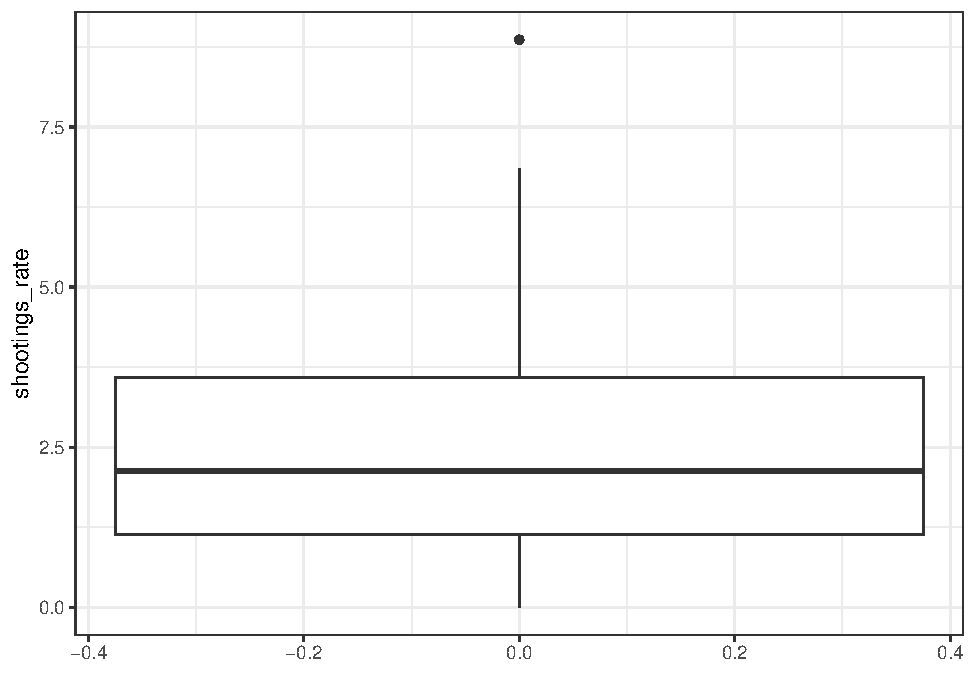
\includegraphics{_main_files/figure-latex/unnamed-chunk-14-1.pdf}

\chapter{Bivariat analys}\label{bivariat-analys}

\section{Krosstabler: Två kategorisk variabler}\label{krosstabler-tvuxe5-kategorisk-variabler}

Precis som alla andra saker i R det finns många olika sätt att skapa kross tabell i R. Här er den enklaste exempel som beräkna bara hur många fall finns det i värj kategori.

\begin{Shaded}
\begin{Highlighting}[]
\FunctionTok{table}\NormalTok{(df}\SpecialCharTok{$}\NormalTok{Radsla\_oro, df}\SpecialCharTok{$}\NormalTok{Storstad)}
\end{Highlighting}
\end{Shaded}

\begin{verbatim}
##              
##               Inte storstad Storstad
##   Inte orolig        140012    60760
##   Orolig             119997    45354
\end{verbatim}

Men vi kan också ändra den kod att räkna ut procent i värj låda

\begin{Shaded}
\begin{Highlighting}[]
\FunctionTok{prop.table}\NormalTok{(}\FunctionTok{table}\NormalTok{(df}\SpecialCharTok{$}\NormalTok{Radsla\_oro, df}\SpecialCharTok{$}\NormalTok{Storstad),}\DecValTok{2}\NormalTok{)}
\end{Highlighting}
\end{Shaded}

\begin{verbatim}
##              
##               Inte storstad  Storstad
##   Inte orolig     0.5384891 0.5725917
##   Orolig          0.4615109 0.4274083
\end{verbatim}

Och vi kan även räkna ut de så att de ser ut som procent

\begin{Shaded}
\begin{Highlighting}[]
\FunctionTok{round}\NormalTok{(}\DecValTok{100}\SpecialCharTok{*} \FunctionTok{prop.table}\NormalTok{(}\FunctionTok{table}\NormalTok{(df}\SpecialCharTok{$}\NormalTok{Radsla\_oro, df}\SpecialCharTok{$}\NormalTok{Storstad),}\DecValTok{2}\NormalTok{))}
\end{Highlighting}
\end{Shaded}

\begin{verbatim}
##              
##               Inte storstad Storstad
##   Inte orolig            54       57
##   Orolig                 46       43
\end{verbatim}

Men nu att räkna ut \(\chi {2}\) vi behöver först räkna ut föväntade värderna om de fanns ingen skillnad mellan grupperna. Formel att räckna ut varje cell i en tabell är \({e}= \frac{radtotal \ast koltotal}{total}\) sen från tabellen övanför det skulle ser ut så här

\begin{Shaded}
\begin{Highlighting}[]
\NormalTok{(}\DecValTok{200772}\SpecialCharTok{*}\DecValTok{260009}\NormalTok{)}\SpecialCharTok{/}\DecValTok{366123}
\end{Highlighting}
\end{Shaded}

\begin{verbatim}
## [1] 142581.9
\end{verbatim}

\begin{Shaded}
\begin{Highlighting}[]
\NormalTok{(}\DecValTok{200772}\SpecialCharTok{*}\DecValTok{106114}\NormalTok{)}\SpecialCharTok{/}\DecValTok{366123}
\end{Highlighting}
\end{Shaded}

\begin{verbatim}
## [1] 58190.06
\end{verbatim}

\begin{Shaded}
\begin{Highlighting}[]
\NormalTok{(}\DecValTok{165351}\SpecialCharTok{*}\DecValTok{260009}\NormalTok{)}\SpecialCharTok{/}\DecValTok{366123}
\end{Highlighting}
\end{Shaded}

\begin{verbatim}
## [1] 117427.1
\end{verbatim}

\begin{Shaded}
\begin{Highlighting}[]
\NormalTok{(}\DecValTok{165351}\SpecialCharTok{*}\DecValTok{106114}\NormalTok{)}\SpecialCharTok{/}\DecValTok{366123}
\end{Highlighting}
\end{Shaded}

\begin{verbatim}
## [1] 47923.94
\end{verbatim}

Sen med förväntade värderna vi kan får \(\chi {2}\) genom formeln\\
\(\chi ^{2}=\sum \frac{(O-E)^2}{E}\)

Och vi kan använder R att räcnka ut \(\chi {2}\) för oss så här:

\begin{Shaded}
\begin{Highlighting}[]
\FunctionTok{chisq.test}\NormalTok{(df}\SpecialCharTok{$}\NormalTok{Storstad, df}\SpecialCharTok{$}\NormalTok{Radsla\_oro)}
\end{Highlighting}
\end{Shaded}

\begin{verbatim}
## 
##  Pearson's Chi-squared test with Yates' continuity correction
## 
## data:  df$Storstad and df$Radsla_oro
## X-squared = 353.74, df = 1, p-value < 2.2e-16
\end{verbatim}

Men vi kan också använder en packet i R som heter sjPlot att visa alla information i samma plats samt kör \(\chi {2}\) prov.

\begin{Shaded}
\begin{Highlighting}[]
\FunctionTok{library}\NormalTok{(sjPlot)}
\end{Highlighting}
\end{Shaded}

\begin{verbatim}
## Warning: package 'sjPlot' was built under R version 4.4.2
\end{verbatim}

\begin{Shaded}
\begin{Highlighting}[]
\FunctionTok{tab\_xtab}\NormalTok{(}
  \AttributeTok{var.row =}\NormalTok{ df}\SpecialCharTok{$}\NormalTok{Radsla\_oro,}
  \AttributeTok{var.col =}\NormalTok{ df}\SpecialCharTok{$}\NormalTok{Storstad,}
  \AttributeTok{show.summary =} \ConstantTok{TRUE}\NormalTok{,}
  \AttributeTok{show.col.prc =} \ConstantTok{TRUE}\NormalTok{,}
  \AttributeTok{use.viewer =} \ConstantTok{TRUE}
\NormalTok{)}
\end{Highlighting}
\end{Shaded}

Radsla\_oro

Storstad

Total

Inte storstad

Storstad

Inte orolig

{140012}{53.8~\%}

{60760}{57.3~\%}

{200772}{54.8~\%}

Orolig

{119997}{46.2~\%}

{45354}{42.7~\%}

{165351}{45.2~\%}

Total

{260009}{100~\%}

{106114}{100~\%}

{366123}{100~\%}

χ2=353.742 · df=1 · \&phi=0.031 · p=0.000

Men då vi kan också skapa en figur av skillnader andel de som är orolig baserad på stads storlek.

\begin{Shaded}
\begin{Highlighting}[]
\NormalTok{df }\SpecialCharTok{\%\textgreater{}\%}
  \FunctionTok{drop\_na}\NormalTok{() }\SpecialCharTok{\%\textgreater{}\%} 
  \FunctionTok{count}\NormalTok{(Storstad, Radsla\_oro) }\SpecialCharTok{\%\textgreater{}\%} 
  \FunctionTok{group\_by}\NormalTok{(Storstad) }\SpecialCharTok{\%\textgreater{}\%}
  \FunctionTok{mutate}\NormalTok{(}\AttributeTok{prop =}\NormalTok{ n }\SpecialCharTok{/} \FunctionTok{sum}\NormalTok{(n), }\AttributeTok{na.rm=}\ConstantTok{TRUE}\NormalTok{) }\SpecialCharTok{\%\textgreater{}\%}
  \FunctionTok{ggplot}\NormalTok{(}\FunctionTok{aes}\NormalTok{(}\AttributeTok{x =}\NormalTok{ Storstad, }\AttributeTok{y =}\NormalTok{ prop, }\AttributeTok{fill =}\NormalTok{ Radsla\_oro)) }\SpecialCharTok{+}
  \FunctionTok{geom\_col}\NormalTok{(}\AttributeTok{position =} \FunctionTok{position\_dodge}\NormalTok{()) }\SpecialCharTok{+}
  \FunctionTok{geom\_text}\NormalTok{(}\FunctionTok{aes}\NormalTok{(}\AttributeTok{label =} \FunctionTok{round}\NormalTok{(}\DecValTok{100} \SpecialCharTok{*}\NormalTok{ prop)),}
            \AttributeTok{position =} \FunctionTok{position\_dodge}\NormalTok{(.}\DecValTok{9}\NormalTok{), }\AttributeTok{vjust =} \SpecialCharTok{{-}}\NormalTok{.}\DecValTok{2}
\NormalTok{  )}\SpecialCharTok{+}
  \FunctionTok{theme\_bw}\NormalTok{()}
\end{Highlighting}
\end{Shaded}

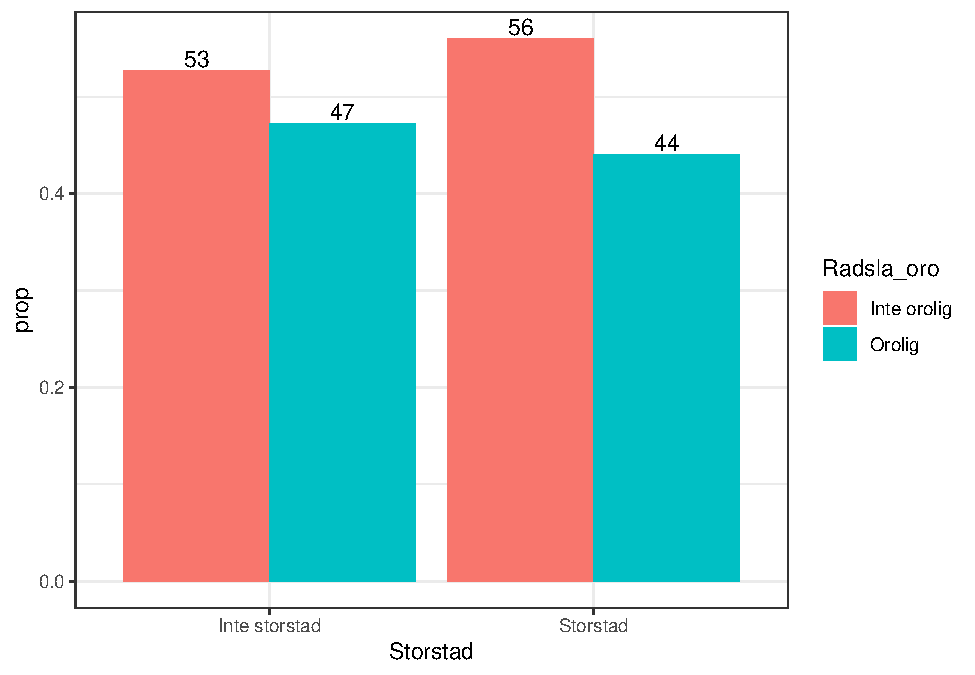
\includegraphics{_main_files/figure-latex/unnamed-chunk-21-1.pdf}

\section{Korrelationer: Två kontinuerlig variabel}\label{korrelationer-tvuxe5-kontinuerlig-variabel}

Bara två variabler från datasetet:

\begin{Shaded}
\begin{Highlighting}[]
\NormalTok{shootings }\SpecialCharTok{\%\textgreater{}\%} 
  \FunctionTok{select}\NormalTok{(shootings\_rate, education\_average) }\SpecialCharTok{\%\textgreater{}\%} \CommentTok{\#Första välja variablerna att inkludera i korrelationsanalys}
  \FunctionTok{tab\_corr}\NormalTok{(}\AttributeTok{corr.method=}\StringTok{\textquotesingle{}pearson\textquotesingle{}}\NormalTok{, }\AttributeTok{triangle =} \StringTok{\textquotesingle{}lower\textquotesingle{}}\NormalTok{)}
\end{Highlighting}
\end{Shaded}

~

shootings\_rate

education\_average

shootings\_rate

~

~

education\_average

0.381**

~

Computed correlation used pearson-method with listwise-deletion.

Sen vi kan kolla på hur alla fyra variabler korrelera med vandra:

\begin{Shaded}
\begin{Highlighting}[]
\NormalTok{shootings }\SpecialCharTok{\%\textgreater{}\%} 
  \FunctionTok{select}\NormalTok{(shootings\_rate, education\_average, trust\_police\_average, income\_average) }\SpecialCharTok{\%\textgreater{}\%} \CommentTok{\#Första välja variablerna att inkludera i korrelationsanalys}
  \FunctionTok{tab\_corr}\NormalTok{(}\AttributeTok{corr.method=}\StringTok{\textquotesingle{}pearson\textquotesingle{}}\NormalTok{, }\AttributeTok{triangle =} \StringTok{\textquotesingle{}lower\textquotesingle{}}\NormalTok{)}
\end{Highlighting}
\end{Shaded}

~

shootings\_rate

education\_average

trust\_police\_average

income\_average

shootings\_rate

~

~

~

~

education\_average

0.381**

~

~

~

trust\_police\_average

-0.151{}

-0.066{}

~

~

income\_average

0.562***

0.565***

-0.184{}

~

Computed correlation used pearson-method with listwise-deletion.

\begin{Shaded}
\begin{Highlighting}[]
\NormalTok{shootings }\SpecialCharTok{\%\textgreater{}\%} 
  \FunctionTok{select}\NormalTok{(shootings\_rate, education\_average, trust\_police\_average, income\_average) }\SpecialCharTok{\%\textgreater{}\%} \CommentTok{\#Första välja variablerna att inkludera i korrelationsanalys}
  \FunctionTok{sjp.corr}\NormalTok{(}\AttributeTok{corr.method =} \StringTok{\textquotesingle{}pearson\textquotesingle{}}\NormalTok{)}
\end{Highlighting}
\end{Shaded}

\begin{verbatim}
## Warning in sjp.corr(., corr.method = "pearson"): 'sjp.corr' is deprecated.
## Please use 'correlation::correlation()' and its related plot()-method.
\end{verbatim}

\begin{verbatim}
## Computing correlation using pearson-method with listwise-deletion...
\end{verbatim}

\begin{verbatim}
## Warning: Removed 10 rows containing missing values or values outside the scale range
## (`geom_text()`).
\end{verbatim}

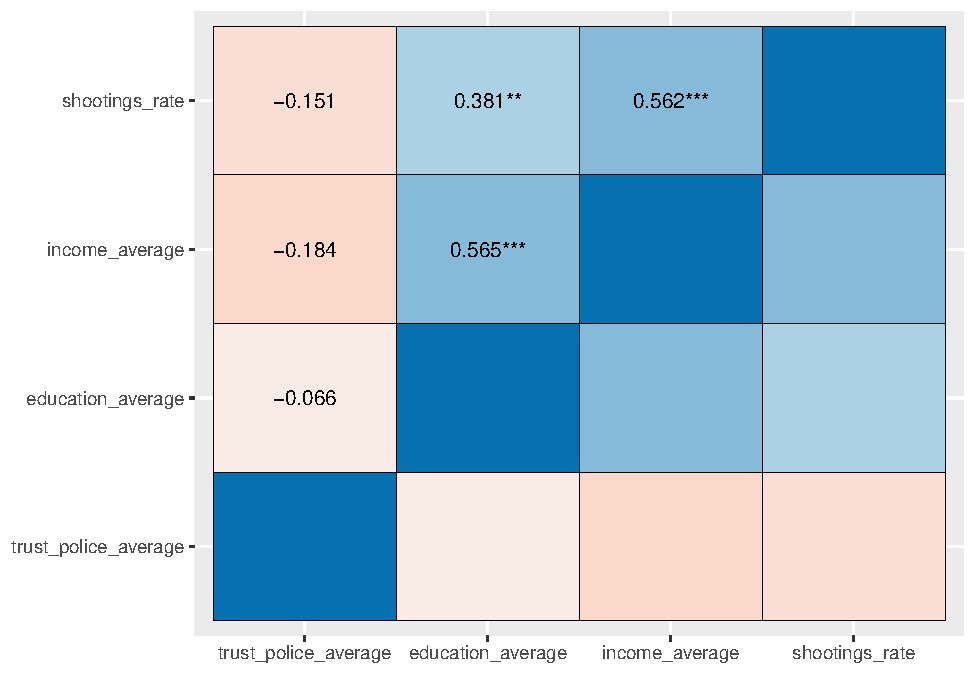
\includegraphics{_main_files/figure-latex/unnamed-chunk-24-1.pdf}

Sen vi kan visualisera sambandet tillsammans med iakttog punkterna med ggplot. Första vi kan bygga en skatterplot av sambandet

\begin{Shaded}
\begin{Highlighting}[]
\NormalTok{shootings }\SpecialCharTok{\%\textgreater{}\%} 
  \FunctionTok{ggplot}\NormalTok{(}\FunctionTok{aes}\NormalTok{(education\_average, shootings\_rate))}\SpecialCharTok{+}
  \FunctionTok{geom\_point}\NormalTok{()}\SpecialCharTok{+}
  \FunctionTok{theme\_bw}\NormalTok{()}
\end{Highlighting}
\end{Shaded}

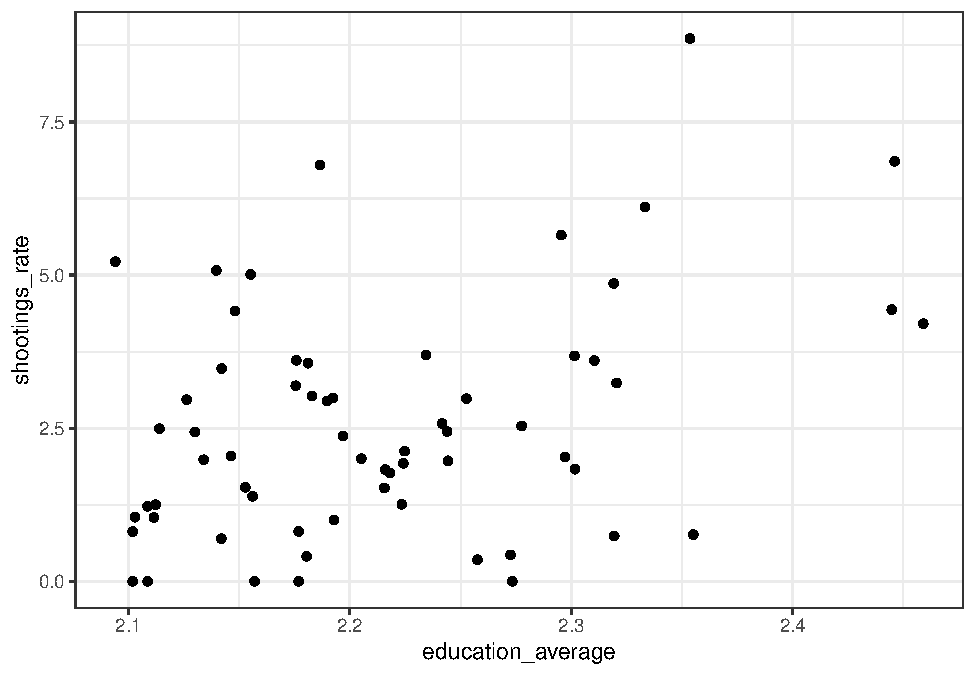
\includegraphics{_main_files/figure-latex/unnamed-chunk-25-1.pdf}
Sen vi kan lägga till en regressions linje

\begin{Shaded}
\begin{Highlighting}[]
\NormalTok{shootings }\SpecialCharTok{\%\textgreater{}\%} 
  \FunctionTok{ggplot}\NormalTok{(}\FunctionTok{aes}\NormalTok{(education\_average, shootings\_rate))}\SpecialCharTok{+}
  \FunctionTok{geom\_point}\NormalTok{()}\SpecialCharTok{+}
  \FunctionTok{geom\_smooth}\NormalTok{(}\AttributeTok{method=} \StringTok{\textquotesingle{}lm\textquotesingle{}}\NormalTok{)}\SpecialCharTok{+}
  \FunctionTok{theme\_bw}\NormalTok{()}
\end{Highlighting}
\end{Shaded}

\begin{verbatim}
## `geom_smooth()` using formula = 'y ~ x'
\end{verbatim}

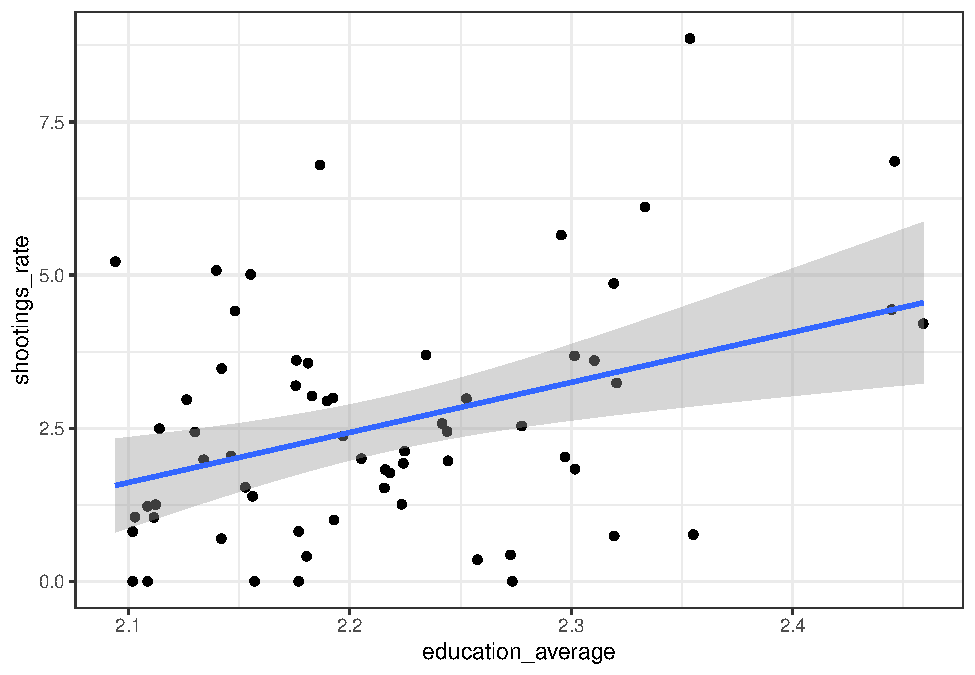
\includegraphics{_main_files/figure-latex/unnamed-chunk-26-1.pdf}

\section{Jämförelsen av medelvärdet: Kontinuerlig beroende varaibel och kategorisk oberoends variabel}\label{juxe4mfuxf6relsen-av-medelvuxe4rdet-kontinuerlig-beroende-varaibel-och-kategorisk-oberoends-variabel}

\begin{Shaded}
\begin{Highlighting}[]
\NormalTok{aov}\OtherTok{\textless{}{-}}\FunctionTok{aov}\NormalTok{(shootings\_rate}\SpecialCharTok{\textasciitilde{}}\NormalTok{ year, }\AttributeTok{data=}\NormalTok{shootings)}
\FunctionTok{summary}\NormalTok{(aov)}
\end{Highlighting}
\end{Shaded}

\begin{verbatim}
##             Df Sum Sq Mean Sq F value Pr(>F)
## year         1   2.97   2.965    0.82  0.369
## Residuals   61 220.51   3.615
\end{verbatim}

Sen vi får medelvärdena och konfidensintervaller men ememans packetet

\begin{Shaded}
\begin{Highlighting}[]
\FunctionTok{library}\NormalTok{(emmeans)}
\end{Highlighting}
\end{Shaded}

\begin{verbatim}
## Warning: package 'emmeans' was built under R version 4.4.2
\end{verbatim}

\begin{verbatim}
## Welcome to emmeans.
## Caution: You lose important information if you filter this package's results.
## See '? untidy'
\end{verbatim}

\begin{Shaded}
\begin{Highlighting}[]
\FunctionTok{emmeans}\NormalTok{(aov, }\AttributeTok{spec =} \StringTok{\textquotesingle{}year\textquotesingle{}}\NormalTok{)}
\end{Highlighting}
\end{Shaded}

\begin{verbatim}
##  year emmean   SE df lower.CL upper.CL
##  2019   2.56 0.24 61     2.08     3.04
## 
## Confidence level used: 0.95
\end{verbatim}

Sen vi kan visualisera sambandet mellan skottfrekvens och år.

\begin{Shaded}
\begin{Highlighting}[]
\NormalTok{shootings }\SpecialCharTok{\%\textgreater{}\%} 
 \FunctionTok{ggplot}\NormalTok{(}\FunctionTok{aes}\NormalTok{(year, shootings\_rate))}\SpecialCharTok{+}
  \FunctionTok{geom\_jitter}\NormalTok{(}\AttributeTok{position=}\FunctionTok{position\_jitter}\NormalTok{(.}\DecValTok{05}\NormalTok{))}\SpecialCharTok{+}
  \FunctionTok{stat\_summary}\NormalTok{(}\AttributeTok{fun.data =}\NormalTok{ mean\_cl\_normal, }\AttributeTok{geom =} \StringTok{"errorbar"}\NormalTok{, }
        \AttributeTok{width =} \FloatTok{0.1}\NormalTok{, }\AttributeTok{position=}\FunctionTok{position\_nudge}\NormalTok{(}\AttributeTok{x =} \FloatTok{0.15}\NormalTok{)) }\SpecialCharTok{+}
    \FunctionTok{stat\_summary}\NormalTok{(}\AttributeTok{fun.y =}\NormalTok{ mean, }\AttributeTok{geom =} \StringTok{"point"}\NormalTok{,}
        \AttributeTok{size =} \DecValTok{3}\NormalTok{, }\AttributeTok{position=}\FunctionTok{position\_nudge}\NormalTok{(}\AttributeTok{x =} \FloatTok{0.15}\NormalTok{))}\SpecialCharTok{+}
  \FunctionTok{theme\_bw}\NormalTok{()}
\end{Highlighting}
\end{Shaded}

\begin{verbatim}
## Warning: The `fun.y` argument of `stat_summary()` is deprecated as of ggplot2 3.3.0.
## i Please use the `fun` argument instead.
## This warning is displayed once every 8 hours.
## Call `lifecycle::last_lifecycle_warnings()` to see where this warning was
## generated.
\end{verbatim}

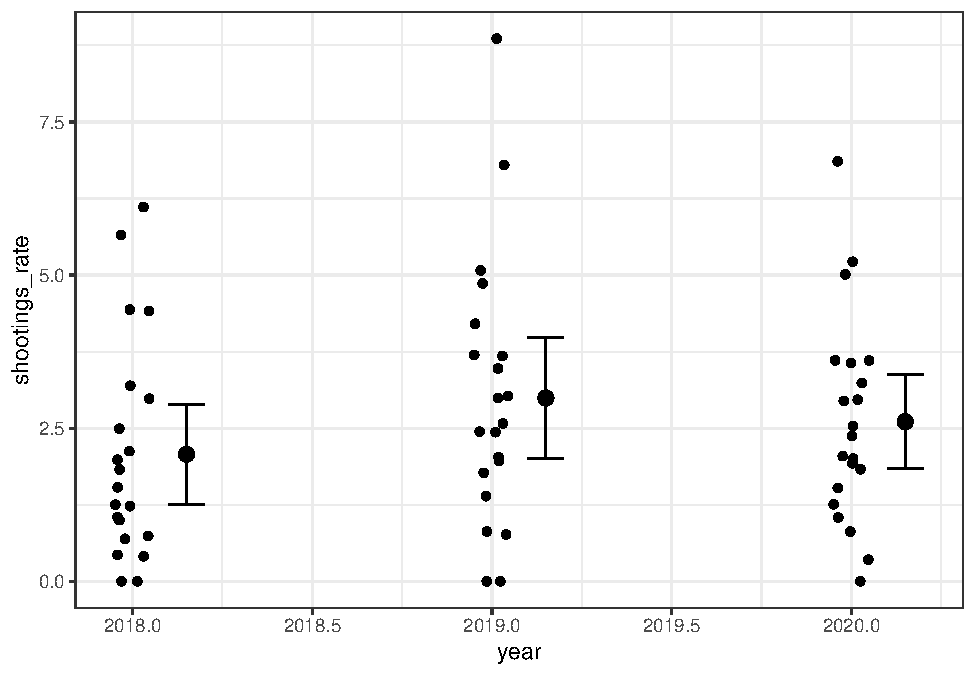
\includegraphics{_main_files/figure-latex/unnamed-chunk-29-1.pdf}

  \bibliography{book.bib,packages.bib}

\end{document}
